\documentclass[12pt, letterpaper]{article}
%\documentclass[12pt, letterpaper]{amsart}

%%%%%%%%%%%% LANGUAGE & ENCODING %%%%%%%%%%%%%%%%%
\usepackage[english]{babel}
\usepackage[utf8]{inputenc}%%%% to process umlauts and accents directly
%\usepackage{indentfirst}
%\usepackage{ucs}

%%%%%%%%%%% PACKAGES %%%%%%%%%%%%%%%%%%%%%%%%%%%%%
% For Hyperlinks
\usepackage[colorlinks,linkcolor=cyan,citecolor=magenta]{hyperref}

% Common math packages
\usepackage{amsthm, amsmath, amsfonts, amssymb, esint, mathrsfs, mathtools}
\usepackage{tensor} % To handle multi-index notation
\usepackage[capitalize,nameinlink]{cleveref} % Nice references
\crefname{equation}{}{} % Removes Eq. from equation references
\numberwithin{equation}{section} % Number equations within each section separately

% Extra symbols
\usepackage{stmaryrd} % contains \owedge  for Kulkarni-Nomizu product and some other special characters
\usepackage{commath} % contains \norm \abs

% Some useful packages
\usepackage{verbatim} %%% enables \begin{comment}    \end{comment}
\usepackage{enumerate} % allows different types of indices
\usepackage{float} % Handling figures

%%%%%%%%%%% MARGINS %%%%%%%%%%%%%%%%%%%%%%%%%%%%%%%%
% Margins
\usepackage[top=1in, bottom=1in, left=1in, right=1in]{geometry}

%%%%%%%%%%% CUSTOM NOTATION  %%%%%%%%%%%%%%%%%%%%%%
\newcommand{\N}{\mathbb{N}}
\newcommand{\Z}{\mathbb{Z}}
\newcommand{\Q}{\mathbb{Q}}
\newcommand{\R}{\mathbb{R}}
\newcommand{\C}{\mathbb{C}}
\newcommand{\K}{\mathbb{K}}

\newcommand{\f}{\mathfrak}
\newcommand{\ul}{\underline}
\newcommand{\mb}{\mathbb}
\newcommand{\mr}{\mathrm}
\newcommand{\mf}{\mathbf}
\newcommand{\mc}{\mathcal}
\newcommand{\e}{\emph}
\newcommand{\vp}{\varphi}
\newcommand{\ve}{\varepsilon}

\newcommand{\vol}{\operatorname{Vol}}
\newcommand{\diam}{\operatorname{diam}}
\newcommand{\dist}{\operatorname{dist}}
\newcommand{\dv}{\operatorname{div}}
\newcommand{\tr}{\operatorname{tr}}

\newcommand{\dd}{\; \mathrm{d}} %%%% d for integration dx
\newcommand{\wt}{\widetilde}
\newcommand{\ol}{\overline}

%%%%%%%%%%% THEOREMS %%%%%%%%%%%%%%%%%%%%%%%%
\newtheorem{theorem}{Theorem}[section]
\newtheorem{lemma}[theorem]{Lemma}
\newtheorem{proposition}[theorem]{Proposition}
\newtheorem{conjecture}[theorem]{Conjecture}
\newtheorem{corollary}[theorem]{Corollary}
\newtheorem{claim}[theorem]{Claim}
\newtheorem{problem}[theorem]{Problem}
\newtheorem{remark}[theorem]{Remark}

\theoremstyle{definition}
\newtheorem{definition}[theorem]{Definition}

\theoremstyle{remark}
\newtheorem{example}[theorem]{Example}


%%%%%%%%%%% TITLE %%%%%%%%%%%%%%%%%%%
%\title[CIS625: Computational Learning Theory]{Computational Learning Theory Lecture Notes}
%\author[Notes by Martin Citoler-Saumell]{Martin Citoler-Saumell}
%\date{Spring 2017}
%\address{University of Pennsylvania\\ Philadelphia, PA 19104}
%\email{\href{mailto:martinci@math.upenn.edu}{martinci@math.upenn.edu}}

\title{Computational Learning Theory Lecture Notes}
\author{Martin Citoler-Saumell}
\date{CIS625 Spring 2017}

%%%%%%%%%%% DOCUMENT BEGINS %%%%%%%%%%%%
\begin{document}

%------------------------------------------------------------
%          LECTURE 9
%------------------------------------------------------------
\section{Lecture 9: 2017.03.27}
Some remarks from last time.
\begin{remark}[Out of sample generalization]
In particular, if we know that $\gamma_t \geq \gamma$, we have that a simpler bound for the training error: $\frac1m\abs{\lbrace i : H(x_i) \ne y_i \rbrace} $. Then if we choose the number of rounds of Adaboosting, $T\geq \frac1{2\gamma^2}\ln(m)$, we can guarantee that $H$ is consistent with the set $S$. Further, if $VCD(\mc H) = d$, then the VCD of $H's$ class is $\leq dT$ (linearity result for VCD-dimension, check the textbook). This means that if we choose $T$ so that $T\geq \frac1{2\gamma^2}\ln(dT)$, then by VCD-theory we have good generalizations out of the sample $S$, i.e. with respect to the true distribution.
\end{remark}

\begin{remark}
Adaboost provides a sort of converse to the following result: ``hypothesis compression'' $\implies$ ``learning''. If we have an algorithm that has a bad relation with the $\ve$ of the PAC-learning model, i.e. it outputs big hypothesis with respect to the error, then we can choose a bigger $\ve$ and feed this ``bad'' algorithm to obtain a much better hypothesis (In fact, sub-linear in $\ve$).
\end{remark}

\subsection*{Today}
\begin{itemize}
\item Learning with queries
\item Algo for DFA
\item PAC "solar system"
\end{itemize}

\subsection{Learning with queries}
\subsubsection*{PAC + Membership Queries}
In essence, it is PAC-learning with a membership query oracle. This gives the algorithm to create ``synthetic'' examples and ask for the true labels. This assumes that there is an underlying ground truth, which might not be true in practice.
\begin{figure}[H]
\centering
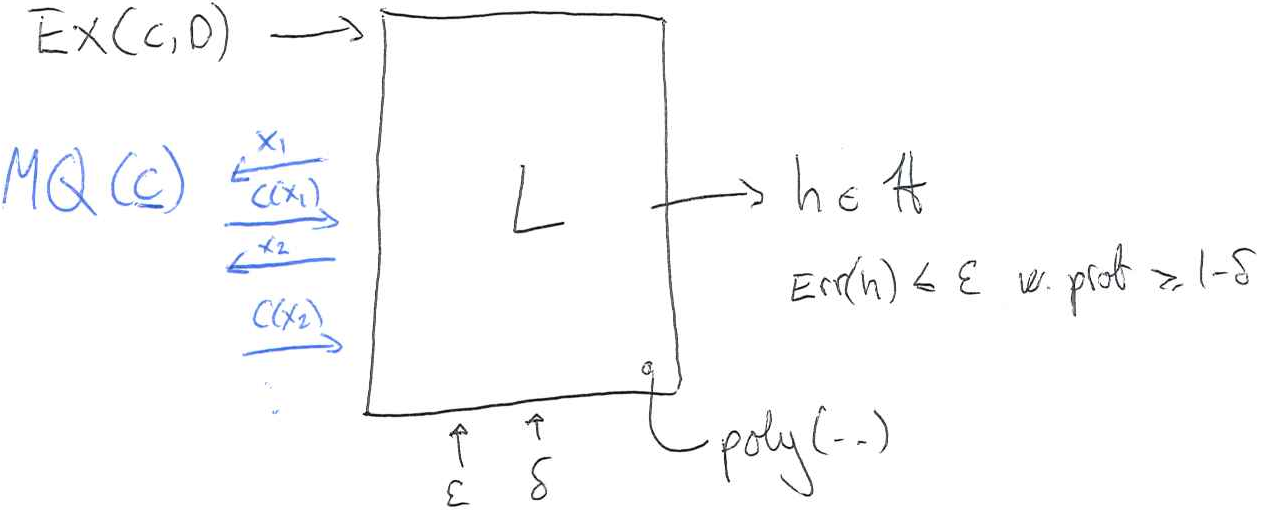
\includegraphics[width=0.6\linewidth]{img/pac-mq.png}
\caption{PAC with membership queries.}
\end{figure}
\begin{remark}
On the surface, adding these membership queries are adding some power to the algorithm that cannot be simulated with $EX(c, D)$ or statistical queries.
\end{remark}
\subsubsection*{Exact Learning with Membership \& Equivalence Queries}
Now consider the following learning model where we have membership queries of individual inputs and an equivalence query oracle that answers whether an hypothesis is the same as the target class (as functions), $c$, and gives \emph{some} counterexample if appropriate i.e. some input where they disagree.
\begin{figure}[H]
\centering
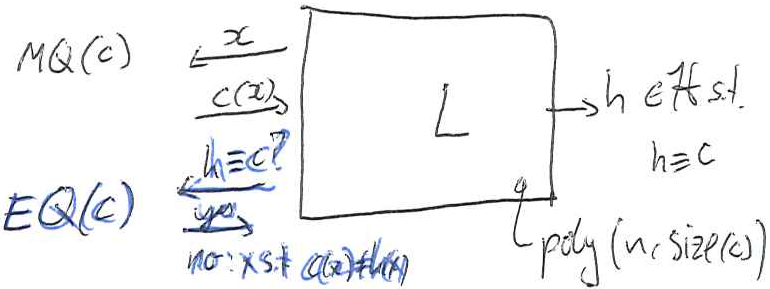
\includegraphics[width=0.6\linewidth]{img/pac-mq-eq.png}
\caption{Exact learning with membership and equivalence queries.}
\end{figure}

\begin{theorem}
If $\mc C$ is exactly learnable from $MQ$ $\&$ $EQ$, then $\mc C$ is PAC+MQ-learnable.
\end{theorem}
\begin{proof}[Sketch of proof.]
We can approximate $EQ$ with enough samples from $EX$. In other words, we sample looking for a counterexample. If we find it great, we can return it. If we don't find it in a reasonable time, then also great because we already have a reasonably good hypothesis.
\end{proof}

\subsubsection{Exact Learning of DFAs in MQ \& EQ (Angluin)}
First of all, recall that PAC-learning DFAs\footnote{Deterministic Finite Automata.}  is provably intractable assuming that factoring is hard.
\begin{example}[DFA]
Consider $X=\lbrace 0, 1\rbrace^*$ with labels $\lbrace +, -\rbrace$. i.e. arbitrary length strings of 1s and 0s. The goal is to learn in poly(size(c), longest counterexample).
\begin{figure}[H]
\centering
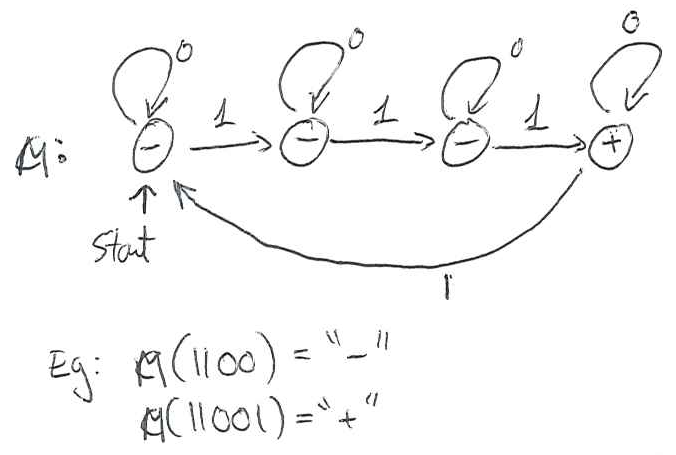
\includegraphics[width=0.6\linewidth]{img/dfa.png}
\caption{Example of DFA.}
\end{figure}
This function is actually $M(x) = +$ if and only if the \#1s in $x$ is $\equiv 3 \mod 4$.
\end{example}

\subsubsection*{Data structure: classification tree T}
To be able to learn DFAs we use a binary tree satisfying the following properties.
\begin{figure}[H]
\centering
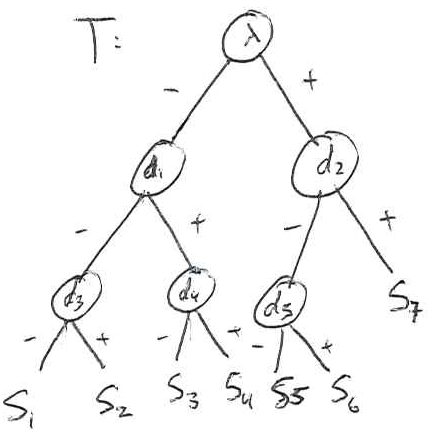
\includegraphics[width=0.3\linewidth]{img/dfa-tree.png}
\caption{Classification tree.}
\end{figure}
\begin{itemize}
\item All the $s$ and $d$ are strings, $\lambda$ is the empty string.
\item Leaves $s$: state access strings.
\item Internal nodes $d$: distinguishing strings.
\item Invariants:
    \begin{enumerate}[i)]
    \item Each $s_i$ reaches a different state of $M$.
    \item For all $s_i$ and $d_j$, $s_i$ is in left/right subtree of $d_j \iff s_id_j$ reaches a $-/+$ state of $M$.
    \end{enumerate}
\end{itemize}

\begin{figure}[H]
\centering
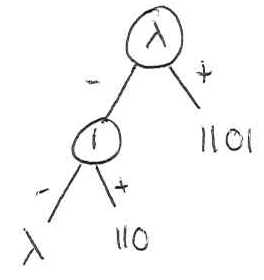
\includegraphics[width=0.3\linewidth]{img/dfa-to-tree.png}
\caption{Classification tree for the example above.}
\end{figure}

\subsubsection*{Learning Model}
\begin{enumerate}
\item MQ on $\lambda$ to get the start state of $\lambda$ i.e. what is the label of the start state, say $+$.
\item EQ on the trivial machine: 
\begin{figure}[H]
\centering
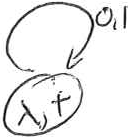
\includegraphics[width=0.1\linewidth]{img/trivial-dfa.png}
\caption{Trivial DFA.}
\end{figure}
    If the machine is not trivial, we obtain a counterexample string, $\langle s, -\rangle$, and we can initialize the tree.
    \begin{figure}[H]
    \centering
    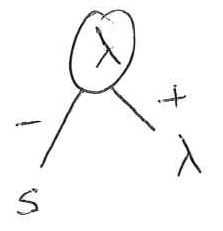
\includegraphics[width=0.1\linewidth]{img/initial-tree.png}
    \caption{Initial classification tree.}
    \end{figure}
\item Now we can iterate this process using equivalence queries and enlarging the tree. But before we can do that we need how to transform a classification tree into a hypothesis DFA and how to make progress on the tree given a new counterexample. 
    \begin{definition}[Sift operation]
    Given a classification tree, $T$, and a string of 1s and 0s, $s$, we define the sift of $s$ by $T$, $\mr{sift}(T,s)$, as the leaf that is reached by the string $s$ in the following way. At each node, we follow the string $s$ and then the string of the node $d_i$ in the true DFA machine and depending on the label of the state we reach, we go left/right down the tree. In the learning model we can actually do this using membership queries. For example:
    \begin{itemize}
    \item At the root, MQ the string $s\lambda$. Say that the query returns $+$, that means we go down the right node.
    \item MQ the string $sd_2$ and suppose the query returns $-$, we go down the left node.
    \item Repeat until we reach a leaf of the tree.
    \end{itemize}
    \end{definition}
    \begin{figure}[H]
    \centering
    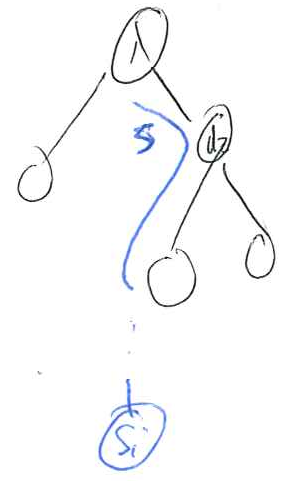
\includegraphics[width=0.1\linewidth]{img/sift-tree.png}
    \caption{Sift operation.}
    \end{figure}
    \begin{remark}~
    \begin{enumerate}[-]
    \item A tree $T$ produces a partition of the space of all strings by labeling each string with $\mr{sift}(T,s)$.
    \item Strings that reach the same state o the true machine must sift to the same leaf. This is because of the properties of the tree mentioned above.
    \end{enumerate}
    \end{remark}
    
    \paragraph{From a tree to a hypothesis machine $\widehat M$.}
    \begin{itemize}
    \item For each leaf of the tree we have a state of the machine.
    \item To obtain the transitions between states we use the sift operation. For example, the state corresponding to the leaf $s_i$ is connected to $\mr{sift}(T, s_i0)$ and  $\mr{sift}(T, s_i1)$.
        \begin{figure}[H]
        \centering
        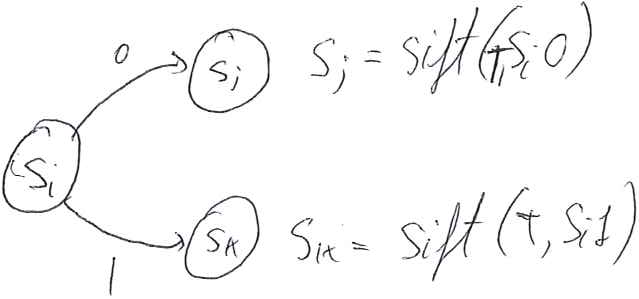
\includegraphics[width=0.2\linewidth]{img/transitions.png}
        \caption{Transitions between states of $\widehat M$.}
        \end{figure}
    \end{itemize}
    
    \paragraph{Making progress on the classification tree.}~\\
    Once we have $\widehat{M}$ we can EQ and either be done or produce a counterexample. Suppose that the equivalence query on $\widehat{M}$ produces the counterexample $\gamma = \gamma_1\gamma_2\ldots\gamma_m$ where $\gamma_l\in\lbrace 0, 1\rbrace$. For simplicity assume that $\gamma$ is $+$ in the true machine $M$ and $-$ in $\widehat{M}$. We use $\gamma$ to improve the classification tree.
    \begin{itemize}
    \item As observed above, our current tree induces a partition of the space of strings, $\lbrace 0, 1\rbrace^*$, and, equivalently, on the states of the machine $M$.
    \item Each of the partition pieces corresponds to one of the current leaves.
    \item We can assume that $S_1 = \lambda$, i.e. that the first leaf tracks the start state of the machine.
    \item Follow $\gamma$ under $\widehat{M}$ and $M$ and see where they diverge. 
    \begin{figure}[H]
    \centering
    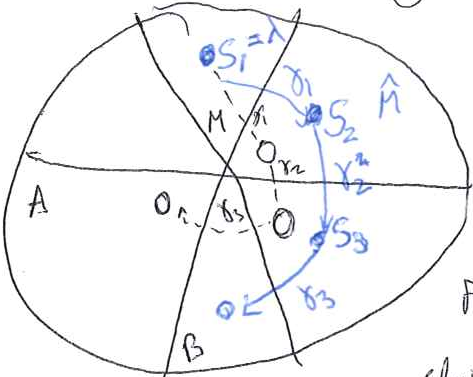
\includegraphics[width=0.3\linewidth]{img/split-criterion.png}
    \caption{Split criterion for leaves.}
    \end{figure} 
    Since they diverge, at some point we must end up  in different equivalence classes which implies that on the step immediately before that we have two different states on the same partition piece. In the figure above, this happens after following $\gamma_1\gamma_2$. Thus, the string $\gamma_1\gamma_2$ reaches a \emph{new state} that used to be in the same equivalence class as $S_3$. We can use this to split the leaf $S_3$.
    \begin{figure}[H]
    \centering
    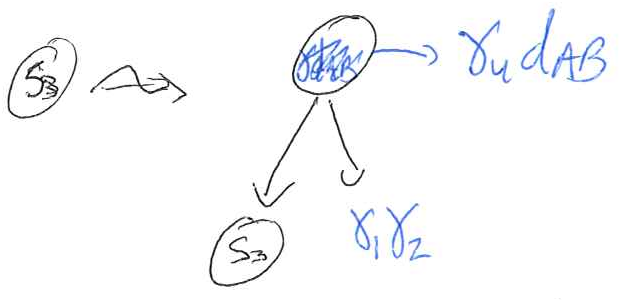
\includegraphics[width=0.3\linewidth]{img/leaf-split.png}
    \caption{Splitting a leaf.}
    \end{figure}       
    where $d_{AB}$ is the distinguishing string of the least common ancestor of the leafs $A$ and $B$, which are also leaves of our tree.
    \end{itemize}
\item The stopping condition is when we have as many leaves as the true machine has states.
\end{enumerate}

\subsection{PAC-learning ``Solar System''}
\begin{figure}[H]
\centering
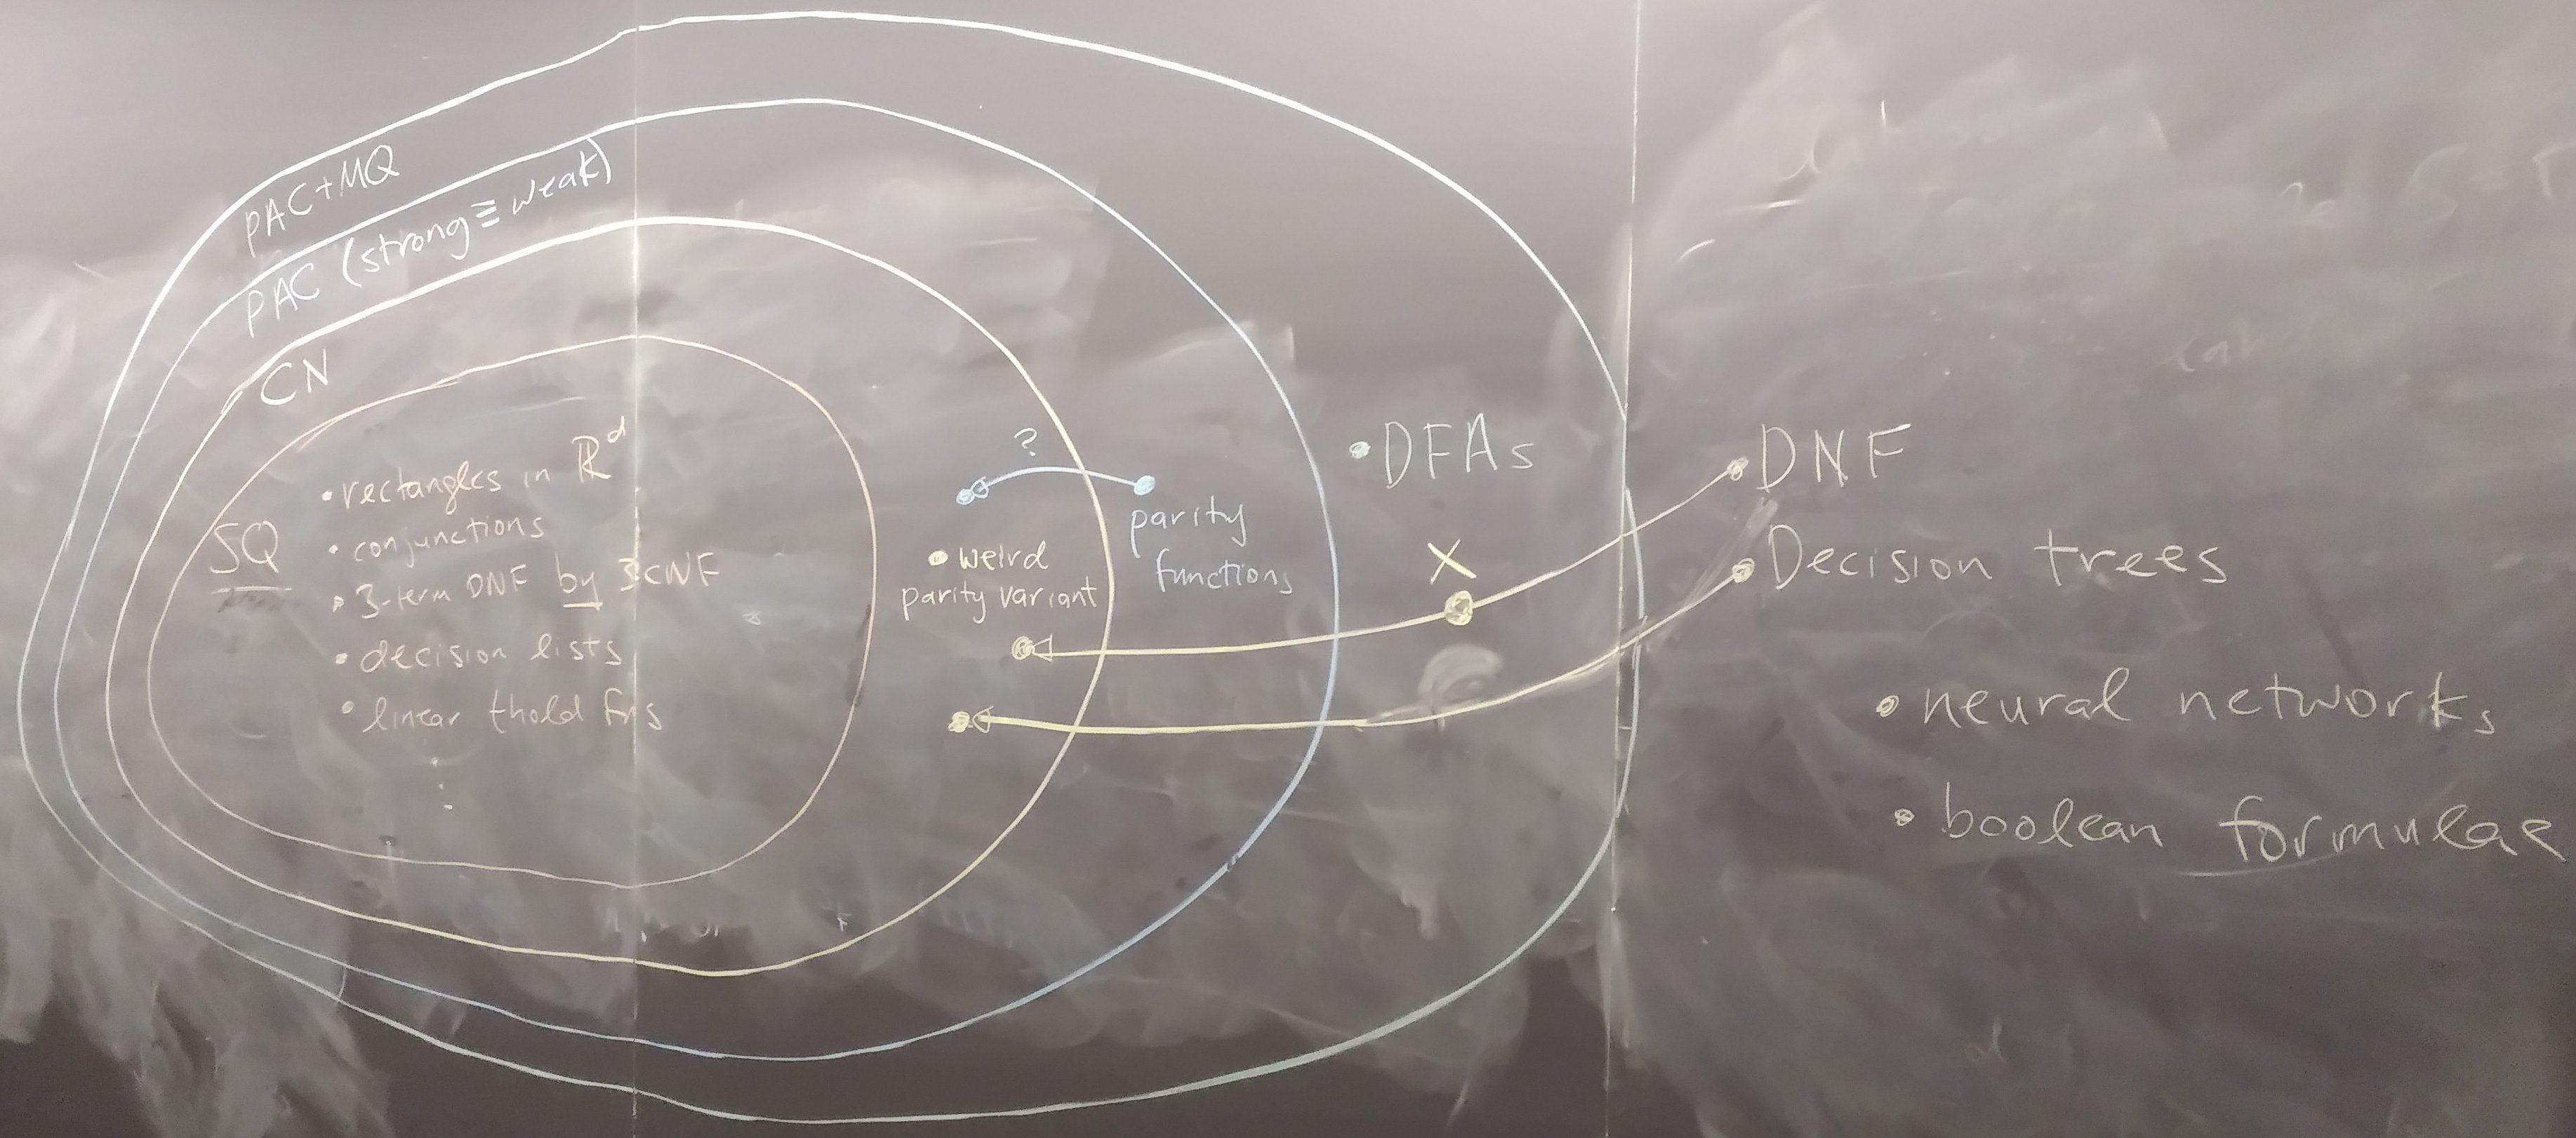
\includegraphics[width=1\linewidth]{img/pac-solar-system.jpg}
\end{figure} 

\end{document}
